\documentclass[tikz]{standalone}
\input{common/tikzBase}
\usetikzlibrary{}
\lstset{
    language=C,
    morekeywords=item,
    style=smaller,
    moredelim={**[is][\btHL<2>]{~2~}{~end~}},
}
\newsavebox{\overExampleACode}
\newsavebox{\overExampleBCode}
\begin{document}
\begin{lrbox}{\overExampleACode}
\begin{lstlisting}
item *load_items(int len) {
  int total_size = ~2~len * sizeof(item);~end~
  if (total_size >= LIMIT) {
    return NULL;
  }
  item *items = malloc(total_size);
  for (int i = 0; i < len; ++i) {
    int failed = read_item(&items[i]);
    if (failed) {
      free(items);
      return NULL;
    }
  }
  return items;
}
\end{lstlisting}
\end{lrbox}
\begin{lrbox}{\overExampleBCode}
\begin{lstlisting}
/* adapted from https://project-zero.issues.chromium.org/issues/42451651 
   Windows Kernel bug! */
char *FormatNumber(char *source, short source_len) {
    unsigned short dest_size = source_len * 6;
    char *dest = malloc(dest_size);
    char *p = dest;
    for (unsigned short i = 0; < source_len; i += 1) {
        *p++ = "0123456789ABCDEF"[*source >> 4];
        *p++ = "0123456789ABCDEF"[*source & 0xF];
        *p++ = ' ';
        source++;
    }
}

\end{lstlisting}
\end{lrbox}

\setSlide{1}
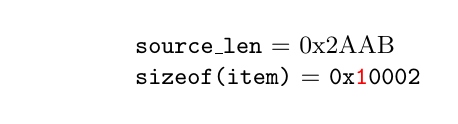
\begin{tikzpicture}
\node[anchor=north east] (code) at (-1,0) {
\usebox{\overExampleBCode}
};
\node[align=left,anchor=north west,font=\small] (t1) at (0,0) {
    {\tt source\_len} = {0x2AAB} \\
    {\tt sizeof(item)} = {\tt 0x{\color{red}1}0002}
};
\end{tikzpicture}
\end{document}
